\documentclass{standalone}
\usepackage{tikz}
\usetikzlibrary{patterns, positioning}
\usepackage[sfdefault]{ClearSans} %% option 'sfdefault' activates Clear Sans as the default text font
\usepackage[T1]{fontenc}

\begin{document}
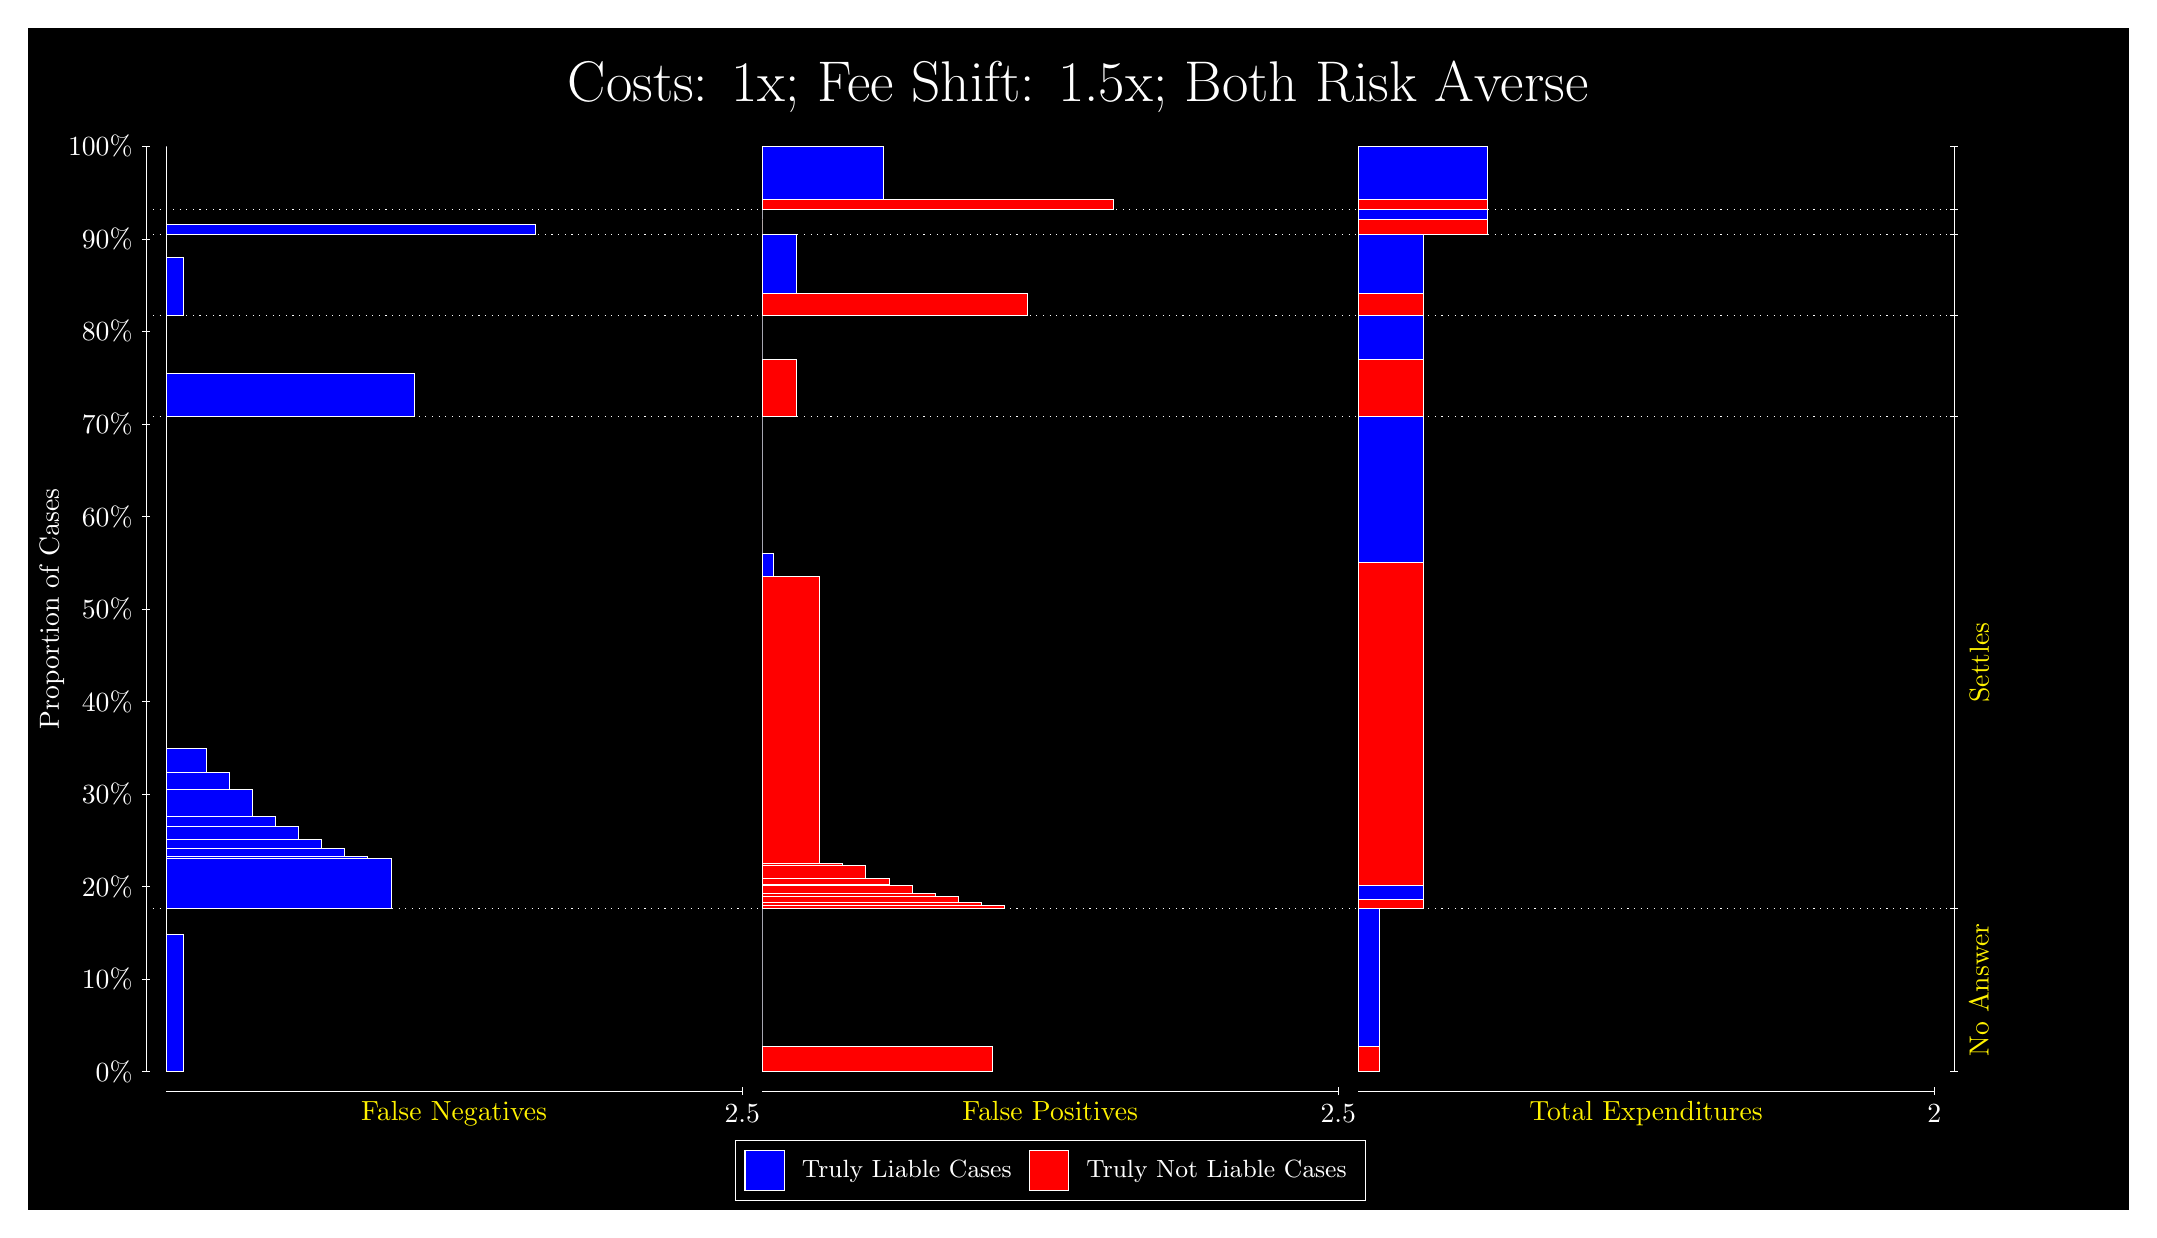
\begin{tikzpicture}
\draw[fill=black] (0,0) rectangle (26.667,15);
\draw[text=white] (0,13.5) rectangle (26.667,15) node[midway] {\huge Costs: 1x; Fee Shift: 1.5x; Both Risk Averse};
\draw[white, very thin] (1.5,1.75) -- (1.5,13.5);
\node[rotate=90, text=white, anchor=center] at (0.3, 7.625) {Proportion of Cases};
\draw[white, very thin] (1.45,1.75) -- (1.55,1.75);
\node[text=white, anchor=east] at (1.45, 1.75) {0\%};
\draw[white, very thin] (1.45,2.925) -- (1.55,2.925);
\node[text=white, anchor=east] at (1.45, 2.925) {10\%};
\draw[white, very thin] (1.45,4.1) -- (1.55,4.1);
\node[text=white, anchor=east] at (1.45, 4.1) {20\%};
\draw[white, very thin] (1.45,5.275) -- (1.55,5.275);
\node[text=white, anchor=east] at (1.45, 5.275) {30\%};
\draw[white, very thin] (1.45,6.45) -- (1.55,6.45);
\node[text=white, anchor=east] at (1.45, 6.45) {40\%};
\draw[white, very thin] (1.45,7.625) -- (1.55,7.625);
\node[text=white, anchor=east] at (1.45, 7.625) {50\%};
\draw[white, very thin] (1.45,8.8) -- (1.55,8.8);
\node[text=white, anchor=east] at (1.45, 8.8) {60\%};
\draw[white, very thin] (1.45,9.975) -- (1.55,9.975);
\node[text=white, anchor=east] at (1.45, 9.975) {70\%};
\draw[white, very thin] (1.45,11.15) -- (1.55,11.15);
\node[text=white, anchor=east] at (1.45, 11.15) {80\%};
\draw[white, very thin] (1.45,12.325) -- (1.55,12.325);
\node[text=white, anchor=east] at (1.45, 12.325) {90\%};
\draw[white, very thin] (1.45,13.5) -- (1.55,13.5);
\node[text=white, anchor=east] at (1.45, 13.5) {100\%};

\draw[white, very thin] (24.457,1.75) -- (24.457,13.5);
\draw[white, very thin] (24.407,1.75) -- (24.507,1.75);
\node[anchor=west] at (24.407, 1.75) {};
\draw[white, very thin] (24.407,3.8188) -- (24.507,3.8188);
\node[anchor=west] at (24.407, 3.8188) {};
\draw[white, very thin] (24.407,10.071) -- (24.507,10.071);
\node[anchor=west] at (24.407, 10.071) {};
\draw[white, very thin] (24.407,11.352) -- (24.507,11.352);
\node[anchor=west] at (24.407, 11.352) {};
\draw[white, very thin] (24.407,12.381) -- (24.507,12.381);
\node[anchor=west] at (24.407, 12.381) {};
\draw[white, very thin] (24.407,12.7) -- (24.507,12.7);
\node[anchor=west] at (24.407, 12.7) {};
\draw[white, very thin] (24.407,13.5) -- (24.507,13.5);
\node[anchor=west] at (24.407, 13.5) {};

\draw[white, very thin, fill=blue] (1.75,1.75) rectangle (1.9696,3.4967);
\draw[white, very thin, fill=red] (1.75,3.4967) rectangle (1.75,3.8188);
\draw[white, very thin, fill=blue] (1.75,3.8188) rectangle (4.6044,4.458);
\draw[white, very thin, fill=blue] (1.75,4.458) rectangle (4.3116,4.4885);
\draw[white, very thin, fill=blue] (1.75,4.4885) rectangle (4.0188,4.5796);
\draw[white, very thin, fill=blue] (1.75,4.5796) rectangle (3.7261,4.6945);
\draw[white, very thin, fill=blue] (1.75,4.6945) rectangle (3.4333,4.8622);
\draw[white, very thin, fill=blue] (1.75,4.8622) rectangle (3.1406,4.9874);
\draw[white, very thin, fill=blue] (1.75,4.9874) rectangle (2.8478,5.3375);
\draw[white, very thin, fill=blue] (1.75,5.3375) rectangle (2.5551,5.5549);
\draw[white, very thin, fill=blue] (1.75,5.5549) rectangle (2.2623,5.8533);
\draw[white, very thin, fill=red] (1.75,5.8533) rectangle (1.75,10.071);
\draw[white, very thin, fill=blue] (1.75,10.071) rectangle (4.8971,10.624);
\draw[white, very thin, fill=red] (1.75,10.624) rectangle (1.75,11.352);
\draw[white, very thin, fill=blue] (1.75,11.352) rectangle (1.9696,12.095);
\draw[white, very thin, fill=red] (1.75,12.095) rectangle (1.75,12.381);
\draw[white, very thin, fill=blue] (1.75,12.381) rectangle (6.4341,12.511);
\draw[white, very thin, fill=red] (1.75,12.511) rectangle (1.75,12.7);
\draw[white, very thin, fill=red] (1.75,12.7) rectangle (1.75,12.833);
\draw[white, very thin, fill=blue] (1.75,12.833) rectangle (1.75,13.5);
\draw[white, very thin, fill=red] (9.3189,1.75) rectangle (12.246,2.0721);
\draw[white, very thin, fill=blue] (9.3189,2.0721) rectangle (9.3189,3.8188);
\draw[white, very thin, fill=red] (9.3189,3.8188) rectangle (12.393,3.8618);
\draw[white, very thin, fill=red] (9.3189,3.8618) rectangle (12.1,3.9039);
\draw[white, very thin, fill=red] (9.3189,3.9039) rectangle (11.807,3.9774);
\draw[white, very thin, fill=red] (9.3189,3.9774) rectangle (11.515,4.0098);
\draw[white, very thin, fill=red] (9.3189,4.0098) rectangle (11.222,4.1173);
\draw[white, very thin, fill=red] (9.3189,4.1173) rectangle (10.929,4.1234);
\draw[white, very thin, fill=red] (9.3189,4.1234) rectangle (10.929,4.2068);
\draw[white, very thin, fill=red] (9.3189,4.2068) rectangle (10.636,4.3674);
\draw[white, very thin, fill=red] (9.3189,4.3674) rectangle (10.344,4.401);
\draw[white, very thin, fill=red] (9.3189,4.401) rectangle (10.051,8.0364);
\draw[white, very thin, fill=blue] (9.3189,8.0364) rectangle (9.4652,8.3348);
\draw[white, very thin, fill=blue] (9.3189,8.3348) rectangle (9.3189,10.071);
\draw[white, very thin, fill=red] (9.3189,10.071) rectangle (9.758,10.799);
\draw[white, very thin, fill=blue] (9.3189,10.799) rectangle (9.3189,11.352);
\draw[white, very thin, fill=red] (9.3189,11.352) rectangle (12.686,11.638);
\draw[white, very thin, fill=blue] (9.3189,11.638) rectangle (9.758,12.381);
\draw[white, very thin, fill=red] (9.3189,12.381) rectangle (9.3189,12.571);
\draw[white, very thin, fill=blue] (9.3189,12.571) rectangle (9.3189,12.7);
\draw[white, very thin, fill=red] (9.3189,12.7) rectangle (13.783,12.833);
\draw[white, very thin, fill=blue] (9.3189,12.833) rectangle (10.856,13.5);
\draw[white, very thin, fill=red] (16.888,1.75) rectangle (17.162,2.0721);
\draw[white, very thin, fill=blue] (16.888,2.0721) rectangle (17.162,3.8188);
\draw[white, very thin, fill=red] (16.888,3.8188) rectangle (17.711,3.9324);
\draw[white, very thin, fill=blue] (16.888,3.9324) rectangle (17.711,4.1145);
\draw[white, very thin, fill=red] (16.888,4.1145) rectangle (17.711,8.2185);
\draw[white, very thin, fill=blue] (16.888,8.2185) rectangle (17.711,10.071);
\draw[white, very thin, fill=red] (16.888,10.071) rectangle (17.711,10.799);
\draw[white, very thin, fill=blue] (16.888,10.799) rectangle (17.711,11.352);
\draw[white, very thin, fill=red] (16.888,11.352) rectangle (17.711,11.638);
\draw[white, very thin, fill=blue] (16.888,11.638) rectangle (17.711,12.381);
\draw[white, very thin, fill=red] (16.888,12.381) rectangle (18.534,12.571);
\draw[white, very thin, fill=blue] (16.888,12.571) rectangle (18.534,12.7);
\draw[white, very thin, fill=red] (16.888,12.7) rectangle (18.534,12.833);
\draw[white, very thin, fill=blue] (16.888,12.833) rectangle (18.534,13.5);
\draw[white, dotted] (1.5,3.8188) -- (24.457,3.8188);
\draw[white, dotted] (1.5,10.071) -- (24.457,10.071);
\draw[white, dotted] (1.5,11.352) -- (24.457,11.352);
\draw[white, dotted] (1.5,12.381) -- (24.457,12.381);
\draw[white, dotted] (1.5,12.7) -- (24.457,12.7);
\draw[white, very thin] (1.75,1.5) -- (9.0689,1.5);
\node[text=yellow, anchor=north] at (5.4094, 1.5) {False Negatives};
\draw[white, very thin] (9.0689,1.45) -- (9.0689,1.55);
\node[text=white, anchor=north] at (9.0689, 1.45) {2.5};

\draw[white, very thin] (9.3189,1.5) -- (16.638,1.5);
\node[text=yellow, anchor=north] at (12.978, 1.5) {False Positives};
\draw[white, very thin] (16.638,1.45) -- (16.638,1.55);
\node[text=white, anchor=north] at (16.638, 1.45) {2.5};

\draw[white, very thin] (16.888,1.5) -- (24.207,1.5);
\node[text=yellow, anchor=north] at (20.547, 1.5) {Total Expenditures};
\draw[white, very thin] (24.207,1.45) -- (24.207,1.55);
\node[text=white, anchor=north] at (24.207, 1.45) {2};

\node[text=yellow, centered, rotate=90] at (24.777, 2.7844) {No Answer};
\node[text=yellow, centered, rotate=90] at (24.777, 6.9448) {Settles};





\draw (12.978300999999998,1.5) node[draw=none] (baseCoordinate) {};
\begin{scope}[align=center]
        \matrix[scale=0.5, draw=white, below=0.5cm of baseCoordinate, nodes={draw}, column sep=0.1cm]{
            \node[rectangle, draw, minimum width=0.5cm, minimum height=0.5cm, fill=blue] {}; &
            \node[draw=none, font=\small, text=white] (B) {Truly Liable Cases}; &
            \node[rectangle, draw, minimum width=0.5cm, minimum height=0.5cm, fill=red] {}; &
            \node[draw=none, font=\small, text=white] (B) {Truly Not Liable Cases}; \\
            };
\end{scope}

\end{tikzpicture}
\end{document}